\documentclass[12pt,a4paper]{article}
\usepackage{amsmath}
\usepackage{graphicx}
\usepackage{geometry}
\usepackage{float}
\geometry{left=2cm,right=2cm,top=2.5cm,bottom=2.5cm}

\title{\textbf{Kinematic and 6-DOF Singularity Analysis Report \\ ($q_7 = -q_1$ Constrained)}}
\author{Automated Generation System}
\date{\today}

\begin{document}
\maketitle

\section{Mathematical Formulation \& Singularity Extraction}
The closed-loop spatial mechanism is driven by $q_1$, with the geometric symmetry explicitly maintained via the constraint $q_7 = -q_1$. To evaluate the structural singularity of the entire mechanism loop, we extract the passive Jacobian $J_p \in \mathbb{R}^{6 \times 6}$ corresponding to the remaining loop kinematics $J_2 \dots J_7$. 

By identifying the local minima of the 6th singular value ($\sigma_6$), the following critical singular configurations (dead centers) were numerically extracted:
\begin{itemize}
    \item Driven by $q_1 = 312.87^\circ$, the minimum singular value drops to $\sigma_6 = 0.000264$.
\end{itemize}

\section{Example Matrix Calculation at $q_1 = 0^\circ$}
The solved full joint configuration (in radians) is:
\begin{equation}
    \mathbf{q} = \begin{bmatrix} 0.0000 \\ 0.0009 \\ 0.0000 \\ -0.0017 \\ -0.0000 \\ -0.0009 \\ -0.0000 \end{bmatrix}
\end{equation}

The full $6 \times 7$ Jacobian matrix $J$:
\begin{equation}
    \resizebox{0.95\textwidth}{!}{$ J = \begin{bmatrix}
  0.000 & 0.000 & -0.000 & 2.500 & -0.002 & -2.500 & 0.000 \\
  0.000 & -1.000 & -0.000 & 3.000 & 0.000 & 2.000 & -0.000 \\
  -0.000 & 0.000 & -3.000 & 0.002 & -0.500 & 0.002 & -2.000 \\
  0.000 & 0.000 & 0.000 & 0.001 & -0.000 & 0.001 & 0.000 \\
  0.000 & 0.000 & -1.000 & -0.000 & -1.000 & -0.000 & 1.000 \\
  1.000 & 1.000 & 0.000 & -1.000 & -0.000 & 1.000 & -0.000
\end{bmatrix} $}
\end{equation}

The structural $6 \times 6$ passive Jacobian $J_p$ (excluding $J_1$):
\begin{equation}
    \resizebox{0.85\textwidth}{!}{$ J_p = \begin{bmatrix}
  0.000 & -0.000 & 2.500 & -0.002 & -2.500 & 0.000 \\
  -1.000 & -0.000 & 3.000 & 0.000 & 2.000 & -0.000 \\
  0.000 & -3.000 & 0.002 & -0.500 & 0.002 & -2.000 \\
  0.000 & 0.000 & 0.001 & -0.000 & 0.001 & 0.000 \\
  0.000 & -1.000 & -0.000 & -1.000 & -0.000 & 1.000 \\
  1.000 & 0.000 & -1.000 & -0.000 & 1.000 & -0.000
\end{bmatrix} $}
\end{equation}

Applying SVD on $J_p = U \Sigma V^T$ yields 6 singular values. The left singular vectors $U$:
\begin{equation}
    \resizebox{0.85\textwidth}{!}{$ U = \begin{bmatrix}
  0.667 & -0.003 & -0.641 & 0.000 & -0.380 & 0.000 \\
  0.671 & 0.001 & 0.738 & -0.000 & -0.068 & 0.000 \\
  0.002 & 0.990 & -0.003 & 0.142 & 0.000 & -0.000 \\
  0.000 & 0.000 & 0.000 & -0.000 & -0.000 & -1.000 \\
  0.000 & 0.142 & -0.001 & -0.990 & 0.000 & 0.000 \\
  -0.324 & 0.001 & 0.210 & -0.000 & -0.923 & 0.000
\end{bmatrix} $}
\end{equation}

The singular values matrix $\Sigma$ ($6 \times 6$):
\begin{equation}
    \resizebox{0.85\textwidth}{!}{$ \Sigma = \begin{bmatrix}
  4.177 & 0.000 & 0.000 & 0.000 & 0.000 & 0.000 \\
  0.000 & 3.669 & 0.000 & 0.000 & 0.000 & 0.000 \\
  0.000 & 0.000 & 3.355 & 0.000 & 0.000 & 0.000 \\
  0.000 & 0.000 & 0.000 & 1.669 & 0.000 & 0.000 \\
  0.000 & 0.000 & 0.000 & 0.000 & 0.892 & 0.000 \\
  0.000 & 0.000 & 0.000 & 0.000 & 0.000 & 0.000
\end{bmatrix} $}
\end{equation}

And $V^T$ ($6 \times 6$):
\begin{equation}
    \resizebox{0.85\textwidth}{!}{$ V^T = \begin{bmatrix}
  -0.238 & -0.002 & 0.959 & -0.001 & -0.155 & -0.001 \\
  0.000 & -0.848 & -0.001 & -0.174 & 0.004 & -0.501 \\
  -0.157 & 0.003 & 0.119 & 0.001 & 0.980 & 0.002 \\
  -0.000 & 0.338 & 0.000 & 0.551 & -0.000 & -0.763 \\
  -0.958 & -0.001 & -0.258 & 0.001 & -0.123 & 0.000 \\
  -0.001 & 0.408 & -0.000 & -0.816 & 0.000 & -0.408
\end{bmatrix} $}
\end{equation}

\section{Analysis Results \& Curve Fitting}
\begin{figure}[H]
    \centering
    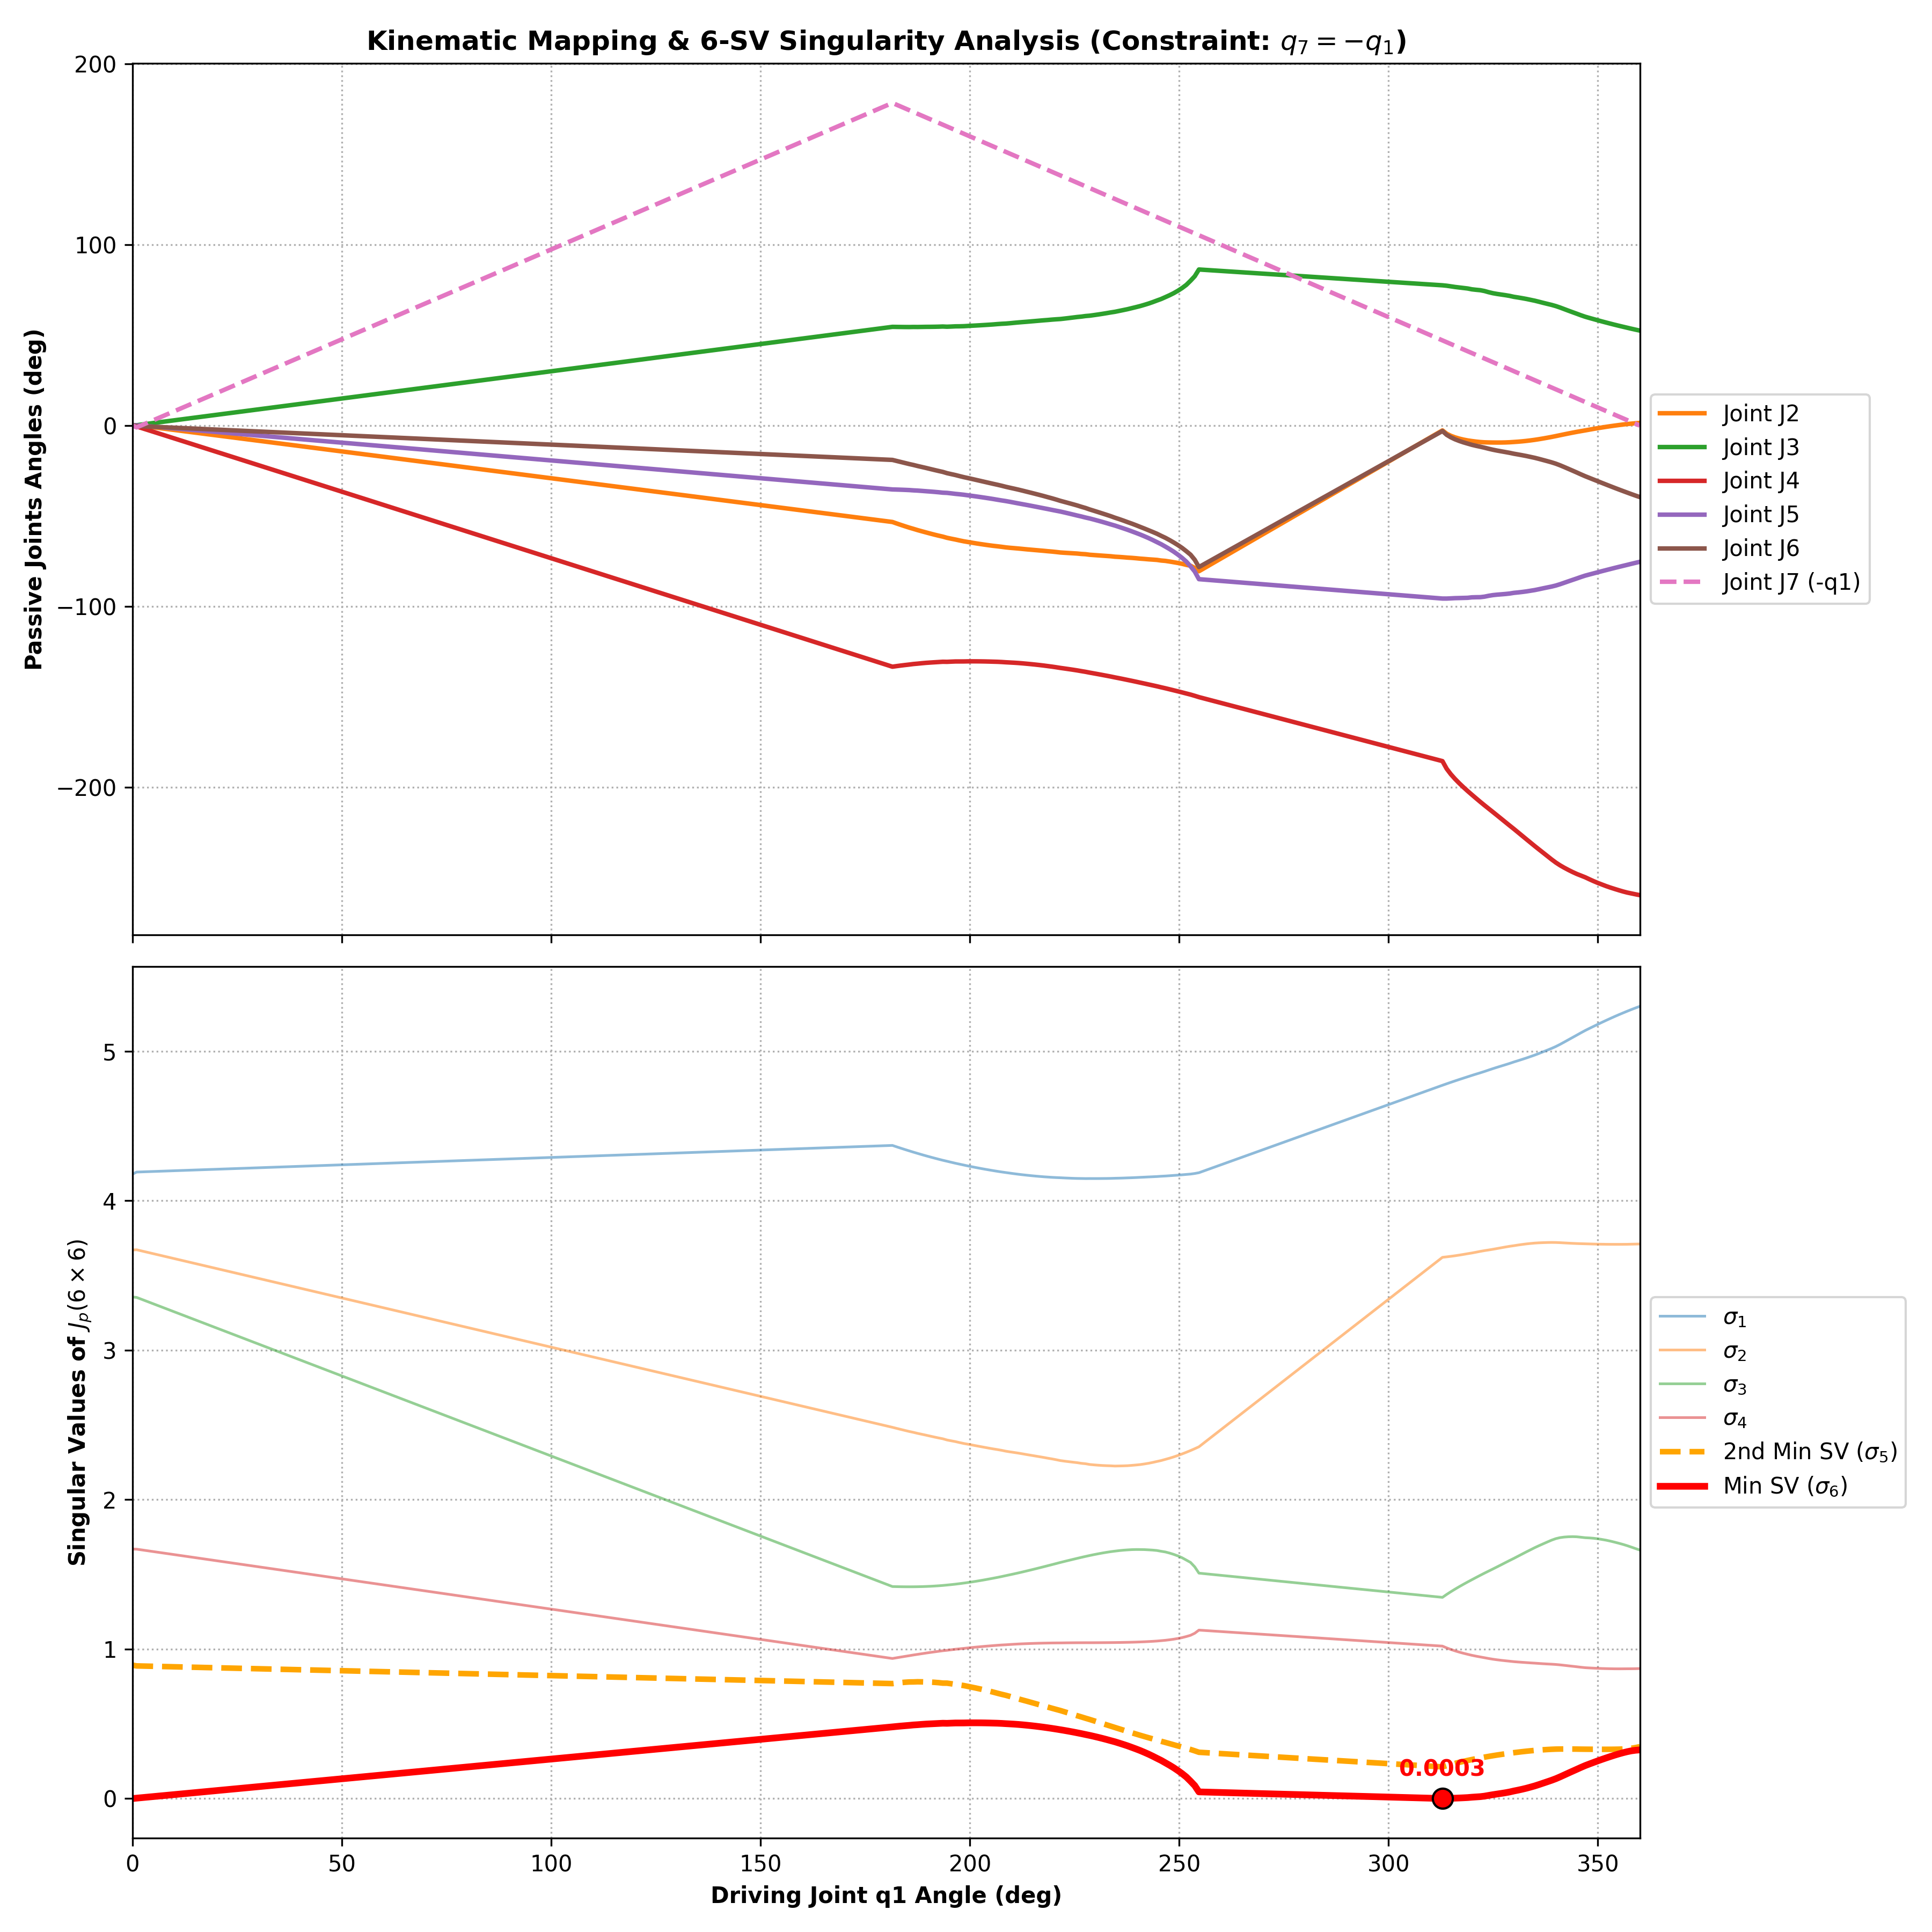
\includegraphics[width=0.9\textwidth]{j1_constrained_6sv_analysis.png}
    \caption{Kinematic mapping and full $6 \times 6$ singular value evolution. Critical dead centers are highlighted in red.}
\end{figure}

The 3rd-order Fourier series expressions for the joints are:
\begin{itemize}
\item \textbf{Joint J2:} \\ $Q_{J2}(x) = +55.136 +34.833\cos(x) +166.434\sin(x) -78.551\cos(2x) -0.346\sin(2x) -7.490\cos(3x) -30.914\sin(3x)$
\item \textbf{Joint J3:} \\ $Q_{J3}(x) = -66.693 -13.783\cos(x) -225.434\sin(x) +108.790\cos(2x) -23.337\sin(2x) +7.051\cos(3x) +36.319\sin(3x)$
\item \textbf{Joint J4:} \\ $Q_{J4}(x) = +270.114 +30.879\cos(x) +719.594\sin(x) -417.467\cos(2x) +90.080\sin(2x) -61.597\cos(3x) -117.017\sin(3x)$
\item \textbf{Joint J5:} \\ $Q_{J5}(x) = +99.266 -0.373\cos(x) +283.813\sin(x) -138.831\cos(2x) +30.306\sin(2x) -11.160\cos(3x) -44.027\sin(3x)$
\item \textbf{Joint J6:} \\ $Q_{J6}(x) = +130.631 +3.319\cos(x) +283.169\sin(x) -149.405\cos(2x) -7.648\sin(2x) -9.840\cos(3x) -61.791\sin(3x)$
\item \textbf{Joint J7 (-q1):} \\ $Q_{J7 (-q1)}(x) = +89.832 -94.932\cos(x) +0.138\sin(x) +0.049\cos(2x) -25.770\sin(2x) +5.241\cos(3x) -0.242\sin(3x)$
\end{itemize}
\end{document}
